\chapter{Cold Electronics}
\label{ch:ce}

\begin{editornote}
  Editor's Note:  This is a new chapter, created from the ``In-Vessel Front-End Electronics'' section formerly in the TPC chapter.
While the old section has been removed from the TPC chapter, some additional ``cleanup'' is still needed there,
to finish removal of CE material that still may be present in the TPC chapter but perhaps no longer belongs there.
\end{editornote}
%
%%%%%%%%%%%%%%%%%%%%%%%%%%%%%%%%
\section{Introduction}
\label{sec:ce-intro}

The TPC read-out electronics are referred to as the ``Cold Electronics" (CE) because they will reside in LAr,
mounted directly on the TPC front-end.
This will minimize channel capacitance and noise by keeping the length of the connection between an anode wire
and its corresponding electronics input to an absolute minimum.
The CE will be implemented as ASIC chips using CMOS technology, which performs well at cryogenic temperatures,
and will provide amplification, shaping, digitization, buffering and multiplexing (Mux) of the signals.
The CE need to be self-triggering because no external trigger will be available for some important measurements,
such as proton decay and supernova bursts.
% since, unlike neutrino-oscillation measurements for which the pulsed beam 
% can provide a trigger for readout, other important measurements, such as proton decay
% and supernova bursts, will have no trigger.  

For each of the 80 APAs in a ten-kton cryostat, one cable bundle will connect to the outside of the cryostat through
a feedthrough, with one feedthrough servicing two APAs.
The bundle consists of wires for low-voltage power, TPC wire-bias voltages, data-out, clock-in,
digital-control IO and an analog-monitoring output.

The scope of the CE subsystem includes the design, procurement, fabrication, testing,
delivery and installation of the CE:
\begin{itemize}
\item Front-end cards installed on the TPC
\item All electronics on those cards
\item Feedthroughs (a single type, henceforth ``signal feedthroughs'') which handle the signal,
low-voltage power, TPC bias voltage, and control lines.
\item External interface crates
\item Power supplies, including low-voltage supplies for the CE and bias-voltage supplies for the TPCs
\item Signal, control, and power cabling between the front-end cards and the feedthroughs
\item Signal, control, and power cabling between the feedthroughs and external power supplies and interface crates
\end{itemize}
This chapter describes the reference design for the CE that meets the required performance for the LBNE liquid argon detector,
LAr-FD.
\begin{editornote}
  The list above is probably not the best way to do this.  However, let's keep it there at least until the TPC chapter has been
  updated to remove unnecessary CE references and information.  Keeping the list (above) will make that a little easier, since the
  list was taken from the old TPC chapter.
\end{editornote}

%
%%%%%%%%%%%%%%%%%%%%%%%%%%%%%%%%
\section{Design Considerations} 
\label{sec:ce-reqs-n-specs}

The requirements for the CE can be found in the requirements documentation \cite{lar-fd-req}.
The most significant ones are the following:

\begin{itemize}	
\item Provide the means to read out the TPCs and transmit their data in a useful format to the Data Acquisition System (DAQ)
\item Operate for the life of the facility without significant loss of function
\item Record the wire-signal waveforms continuously without dead time
\item Use only materials that are compatible with high-purity liquid argon
\item Provide sufficient precision and range in the digitization to:
\begin{itemize}
\item Discriminate electrons from photon conversions
\item Optimize for high- and low-energy tracks from accelerator-neutrino interactions
\item Distinguish a Minimum Ionizing Particle (MIP) from noise with a signal-to-noise ratio $>$ 9:1
\item Measure the ionization up to 15 times that of a MIP particle;
this is necessary to identify stopping kaons from proton decay
\end{itemize}
\item All power supplies:
\begin{itemize}
\item Will be monitored and controlled locally
\item Will be monitored and controlled remotely through the DAQ system
\item Will have over-current and over-voltage protection circuits
\item Will have an output-voltage ripple less than 10\% of the equivalent thermal noise from the front-end electronics
\end{itemize}
\item The power supplies for the wire-plane bias voltages must provide sufficient current.
\item The low-voltage (signal) feedthroughs must be able to withstand twice their nominal operating voltages 
with a maximum specified leakage current in 1-atm argon gas, and must be able to deliver sufficient DC current.
\end{itemize}

\begin{editornote}
  Again, the list above is may not be the best way to do this.
  However, let's keep it there at least until the TPC chapter has been
  updated to remove unnecessary CE references and information.
  Keeping the list (above) will make that a little easier, since the list was taken from the old TPC chapter.
\end{editornote}

%
%%%%%%%%%%%%%%%%%%%%%%%%%%%%%%%%
\section{Architecture}
\label{sec:fe-arch}

Figure~\ref{fig:ce-elec-schematic} shows the CE architecture that meets the requirements for the LAr-FD TPC.
Except for the Digital ASIC, this has already been prototyped and tested,
using a commercial FPGA to perform the r\^ole of the Digital ASIC.  
The Cold Front End Motherboard Assembly (CMB) consists of an Analog Mother Board with a Digital ASIC Mezzanine.  

The Analog Motherboard is instrumented as a 128 channel board which uses eight 16-channel FE ASICs and
eight 16-channel ADC ASICs as well as low voltage regulators.
The 16-channel FE ASIC provides amplification and pulse shaping.
The 16-channel ADC ASIC provides a 12 bit digitizer, local buffering and an 8:1 Mux stage with two serial readout lines in parallel.

The Digital ASIC Mezzanine provides the board space for the Cold Digital Data ASIC (COLDATA) and required voltage regulators.
The COLDATA ASIC provides the communication protocol with the warm data acquisition system (DAQ),
the control required to download and readout the FE and ADC ASICs,
the system clock interface and the data links and drivers to DAQ.
The COLDATA ASIC will also provide up to four high speed links capable of driving 1~Gbps each.
This will provide sufficient bandwidth for all the data (3.072~Gbps) plus an encoding scheme and frame data.
Data will be driven off-board to DAQ through use of copper cable utilizing low-voltage differential signaling (LVDS).
Output data cables will go to a signal feedthrough and from there to an external crate mounted nearby.
Under DAQ scope, further data processing is done and data is transmitted via optical fiber to front-end computers.

Each APA is instrumented with 20 CMBs, for a total of 2,560 channels per APA.
Because each CMB is read out separately and in parallel with all others,
the data rates will not be high enough to require the use of optical fibers in the cold,
nor is there a need for zero-suppression or data compression.

\begin{editornote}
  Data rate will be 256~ch$\times$12~bits/ch every 500~ns for a rate of 3.072~Gbps.
  With 8B10B encoding this is 3.84~Gbps, plus there will be some overhead for frame data.
  This gives us a conservative rate of 1~Gbps per link, which can possibly increase to 2~Gbps
  in the future if we find the design and cabling can support that rate.

  Also note, we should put a picture of the actual FE board assembly into the CDR to show progress.

  We need to be consistent in how we refer to ASICs -- I have tried to use FE ASIC, ADC ASIC and COLDATA ASIC.
  --Terri
\end{editornote}

Figure~\ref{fig:ce-elec-asic-layout} shows a block diagram of the proposed 16-channel front-end ASIC.
Each channel includes a charge amplifier with a gain selectable from one of 4.7, 7.8, 14 and 25~mV/fC
(full scale charge of 55, 100, 180 and 300~fC),
a high-order anti-aliasing filter with adjustable time
constant (peaking time 0.5, 1, 2, and 3 $\mathrm{\mu}$s),
an option to enable AC coupling,
and a baseline adjustment for operation with either the collecting or the non-collecting wires.
The 16-channel FE ASICs then transmit the shaped pulse to a 12-channel 12-bit 2~MS/s ADC ASIC.
Shared among the 16 channels are the bias circuits, programming registers,
a temperature monitor, the digital multiplexer (8:1),
an analog buffer for signal monitoring, and the digital interface.
A 600-kb buffer is included in this design, capable of storing a 1.5-ms 
event sampled at 2~MS/s in each channel.
The estimated power dissipation is below 15~mW per channel at 1.8~V supply.

\begin{editornote}
  Should we get separate power numbers for FE and ADC ASICs? --Terri

  I don't think that is necessary.  Total power is all that matters in the CDR.  -- RWH.
\end{editornote}

\begin{figure}[htbp]
\centering
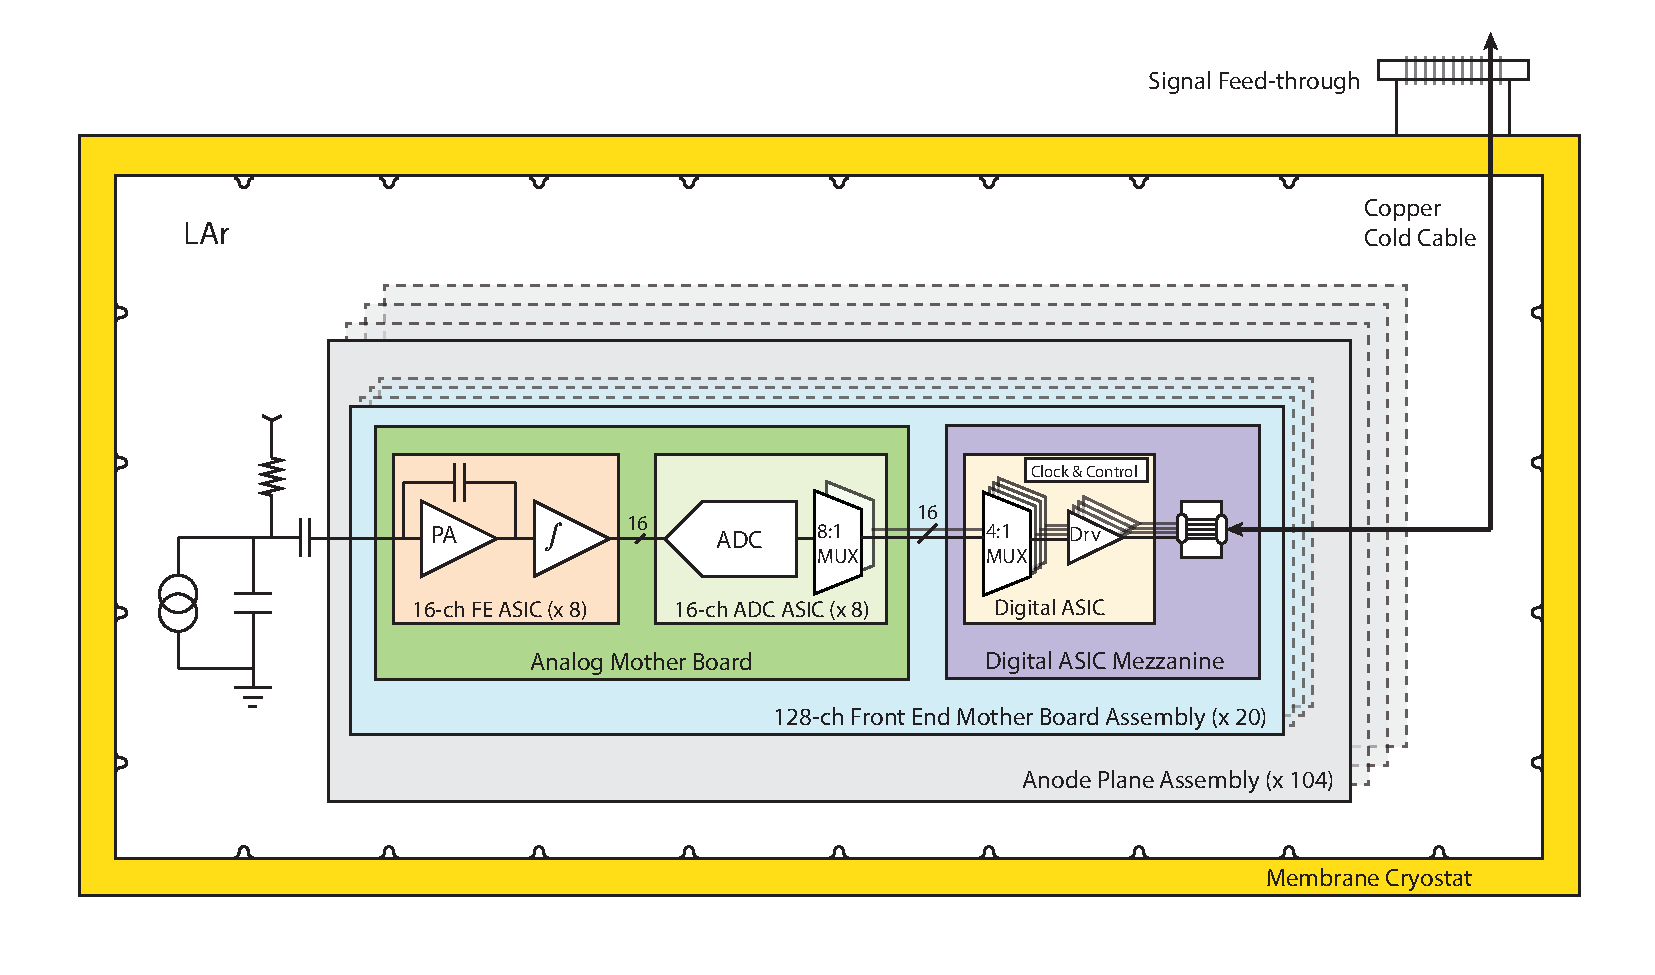
\includegraphics[width=\linewidth]{elect_schem.pdf}
\caption{
  The CE Architecture.
  The basic unit is the 128-channel Front End Mother Board Assembly, also referred to as the Cold Mother Board (CMB).
  Each APA has 20 CMBs installed on its front end for a total of 2,560 channels per APA.
}
\label{fig:ce-elec-schematic}
\end{figure}
\begin{figure}[htbp]
\centering
\includegraphics[width=\linewidth]{v5c3-cel-ASIC-layout}
\caption{Architecture and layout of the 16-channel front-end mixed-signal ASIC}
\label{fig:ce-elec-asic-layout}
\end{figure}

%
%%%%%%%%%%%%%%%%
\subsection{Data Rates}
\label{subsec:fe-arch-rates}

For neutrino-oscillation measurements the pulsed beam could provide a
trigger for readout, but for other measurements, such as proton decay
and supernova bursts, there will be no trigger.
Therefore the APAs will be self triggering, and the
data rates will dependend on the event rates for background processes.
Dominant backgrounds are decays of radionuclides in the LAr, predominantly the naturally occurring Ar$^{39}$.
The cosmic-muon rate at the 4850 Level is approximately 2.3~mHz per APA.
Reading an APA (2,560 wires) for one drift time (4,625 samples) gives 142~Mb of data.
At the cosmic-event rate, the net data rate is 0.3~Mb/s per APA.
For radioactive decay of Ar$^{39}$ the rates are much higher: the specific activity is 1~Bq/kg which results in 183~kHz/APA.
At this rate, the APA will be continuously read out,
at a data rate of 1.5~Gb/s on each of its 40 parallel outputs;
of course, since the ionization produced by these events is highly localized,
most of the drift ``frame'' is empty.
The mean range of the beta from Ar$^{39}$ decay is only 0.3~mm, so all
of the signal is contained in a single over-threshold-sample of a single wire, for a true ``information''
rate of 0.6~Mb/s.

% In order to
% reduce the rate (and volume) of recorded data to tolerable values, 
% data buffering must be provided.
% The simplest scheme is to do this at the APA level, deriving
% a write-enable from the logic OR of discriminators on all the charge
% collecting (Y) wires in an APA, and then writing all data to a buffer
% while the write-enable is true.
% Baseline samples could be recorded
% with reduced range (four bits) and compacted into full words.
% This mode would still record large volumes of data without useful
% information, particularly for simple event topologies and from low-energy 
% events (radioactive decays) and noise. 

%
%%%%%%%%%%%%%%%%
\section{CMOS Circuit Design}
\label{sec:fe-CMOS}

\begin{editornote}
  I think the ``CMOS 0.25~$\mu$m'' (etc.) needs to be updated.
\end{editornote}
To successfully design CMOS circuits that will operate at cryogenic 
temperatures, two critical issues must be addressed and resolved. 
The first issue is the need for realistic models at the operating temperature 
of all active and passive components in order to reliably predict operating points,
signal response, and noise during the design process.
The second issue is that the design must ensure a long operational lifetime, since once the TPC is filled 
with LAr the detector must operate for about 15~years without any access to the 
electronics for repair or replacement.
Concerning the availability of realistic models, 
our preliminary results from the cryogenic characterization (down to 40 K) of a complete 
mixed-signal ASIC \cite{CMOS-Compton} in a commercial CMOS 0.25~$\mu$m technology, 
originally developed for room-temperature applications, indicates that the models 
are useful to first order.
To refine these models, several 
single-transistor test structures were fabricated on the first prototype of the 0.18~$\mu$m device. 
Measurements of the properties of these structures at cryogenic temperatures 
have been used to refine the device models at 89~K. 
\begin{editornote}
  Should we spell out in some small detail our plan for developing models?
  Or does that belong in the Digital ASIC section, along with our plan for developing libraries?
\end{editornote}

The lifetime of CMOS circuits is limited by several mechanisms which degrade 
the performance over time, eventually causing the circuit to fail to perform as specified. 
The rates of most degradation mechanisms in CMOS, such as electro-migration (EM), 
stress migration (SM), time-dependent dielectric breakdown (TDDB), thermal cycling (TC), 
and negative bias-temperature instability (NBTI), all scale with temperature such that 
cryogenic operation is favored \cite{CMOS-lifetime}\cite{PMOS-model}. The only mechanism 
that could affect the lifetime at cryogenic temperature is the degradation due to 
impact ionization, which causes charge trapping in the MOSFET gate oxide at 
large drain-current densities (the ``Hot Carrier'' effect). Results from a CMOS reliability study~\cite{CMOS-reliability} 
provide general design guidelines (for device geometry, bias and current density) 
that should guarantee a lifetime well in excess of 15~years for continuous cryogenic operation. 
These design guidelines also provide information for designing test conditions to observe the 
deterioration mechanism and to extrapolate from accelerated deterioration rates, 
measured under stressed conditions within practical times, to the ultimate lifetime under normal operation.

A monitor of the impact ionization is the bulk current, which reaches a maximum at $V_DS = V_DD$ and at $V_GS = 0.5 V_DD$. 
When operating constantly in this condition at room temperature, a properly designed device 
will typically have a lifetime (defined as a 10\% degradation in $g_m$) of about 10~years. 
The bulk current (i.e., the impact ionization) increases by roughly a factor of four from 300~K to 77~K 
\cite{CMOS-reliability} and a circuit designed for operation at room temperature would have 
a proportionately shorter useful life at cryogenic temperature. As stated above, in order to guarantee 
the required lifetime at cryogenic temperatures, design guidelines must be modified for both analog 
and digital circuits. For analog circuits, this is done by operating the devices at moderate-to-low 
drain current densities, where impact ionization becomes negligible. For digital circuits, 
operating the devices with reduced $V_DD$ (about 20\%) and using non-minimum channel length L, 
which is easily accommodated since at cryogenic temperature the speed of the digital circuit increases, 
compensating for the increased L. These guidelines will be verified with accelerated aging tests, 
at increasing values of $V_DD$, on dedicated structures. Such tests also will be conducted on 
prototype samples throughout the development process to verify the long-term reliability of the final ASICs.

%
%%%%%%%%%%%%%%%%
\subsection{Cold Analog ASICs}
\label{subsec:fe-CMOS-analog}

The development of the readout ASIC has begun by designing and fabricating in a commercial CMOS
process (0.18~$\mu$m and 1.8V) a 16-channel
ASIC implementing the complete analog front-end section of the scheme shown in Figure~\ref{fig:ce-elec-asic-layout}. 
This process is expected to be available for at least another 10~years. 
The charge amplifier input MOSFET is a p-channel biased at 2~mA with a L/W (channel length/width) ratio
of 0.27~$\mu$m / 10~mm, followed by dual cascade stages.
The charge amplification and shaping filter have
digitally programmable gain and peaking time as described above.
Each channel also implements a high-performance output driver which, in the
final version, will be replaced with a sample-and-hold stage preceding the ADC.
The ASIC integrates a band-gap reference (BGR)  to generate all the internal bias voltages and currents.
This guarantees a high stability of the operating point over a wide range of
temperatures, including cryogenic.
The ASIC is packaged in a commercial, fully encapsulated plastic QFP 80 package.

This ASIC has now been through four design/fabrication/testing revision cycles.
Prototypes from each cycle have been evaluated and characterized at room (300~K) and liquid nitrogen (77~K) temperatures.
During these tests the circuits have been cycled multiple times
between the two temperatures and operated without any change in performance.
Figure~\ref{fig:ce-elec-shaper-out} shows the measured pulse response, along with
details on the adjustability of the gain, peaking time and baseline.
These results are in close agreement with the simulations and indicate
that both the analog and the digital circuits and interface operate as
expected in a cryogenic environment.
Simulations and experimental results show that the pole-zero cancellation needs to be optimized,
which will be done in the next revision of the design.
Also reported in Figure~\ref{fig:ce-elec-shaper-out} are the outputs of the BGR and temperature sensor,
which are in close agreement with the simulations as well.

\begin{figure}[htbp]
\centering
\includegraphics[width=\linewidth]{v5c3-cel-shaper-out.pdf}
\caption[Measured pulse response with details]{Measured pulse response with details on gain, peaking time and baseline adjustments}
\label{fig:ce-elec-shaper-out}
\end{figure}

\begin{figure}[htbp]
\centering
\includegraphics[width=4in]{v5c3-cel-enc.pdf}
\caption[Measured ENC vs filter time constant]{Measured ENC vs filter time constant from the first two versions of the analog front end ASICs}
\label{fig:ce-elec-enc}
\end{figure}

Figure~\ref{fig:ce-elec-enc} shows the measured ENC versus filter-time constant (peaking time).
At 1~$\mu$s about 650 e$^{-}$ was measured,
to be compared to the simulated value of 500 e$^{-}$. The difference is
mainly due to the thermal noise from a $\sim$
11-ohm parasitic resistance of the input
line (shown in the detail of Figure~\ref{fig:ce-elec-enc}), which contributes about 350
electrons at 77~K. The width of the line will be increased in a
revision in order to make this contribution negligible. A second
contribution, on the order of 100 e$^{-}$, was due to the dielectric
loss from the  capacitor (220~pF) used to simulate the wire (the cases of MICA and NPO ceramic were compared). This contribution would not be
present with the input connected to a sense wire in the TPC.

Each channel is equipped with an injection capacitor which can be used
for test and calibration and can be enabled or disabled through a
dedicated register. The injection capacitance has been measured using 
a calibrated external capacitor. The measurements show
that the calibration capacitance is extremely stable, changing from
184~fF at room temperature to 183~fF at 77~K. This result and the measured
stability of the peaking time demonstrate the high stability of the
passive components with the temperature. Channel-to-channel and chip-to-chip
variation in the calibration capacitor are typically less than 1\%. Measurements are being carried
out on the individual test structures fabricated on this ASIC to
confirm device models and design guidelines.

%
%%%%%%%%%%%%%%%%
\subsection{Cold Digital ASICs}
\label{subsec:fe-CMOS-digital}

The development of the COLDATA ASIC will follow the general guidelines developed for the cold analog ASICs.
The COLDATA design will differ from the analog design in a couple of aspects.
It is anticipated that the digital ASIC will make use of a 65~nm CMOS technology and require a
digital library with accurate cold timing models allowing for high level language design and
automated place and route for design blocks using extensive digital logic.  

\begin{editornote}
  Need a caption for the COLDATA figure, and the fonts need to be larger.
\end{editornote}
\begin{figure}[htbp]
\centering
\includegraphics[width=4in]{elec-COLDATAfig.pdf}
\caption{Add a caption here.}
\label{fig:elec-COLDATAfig}
\end{figure}
A block diagram of the COLDATA is presented in Fig.~\ref{fig:elec-COLDATAfig}.
The major components of COLDATA include a downlink which is required to receive the system clock and
the control/download information transmitted from the DAQ.
The download data must be transmitted to the FE and ADC ASICs on the CMB.
The system clock will provide a frequency-reference to a crystal based Phase Lock Loop (PLL)
which will generate a low jitter stable clock to the high speed serializer. 

A single COLDATA on each CMB will also be receiving the data from each of the eight ADCs on board.
Each ADC will transmit two streams of data at 192~Mbps for a total data input of 3.072~Gbps.
All data will be transmitted off board.
It is anticipated that an encoding scheme, such as 8B10B, will be used and
some frame data will be added to indicate event blocks.
Thus, it is planned to drive four 1~Gbps links from each COLDATA.
A line driver will be designed which is capable of driving a copper link for the approximate 20~m required
to exit the LAr environment. 

%
%%%%%%%%%%%%%%%%%%%%%%%%%%%%%%%%
\section{Signal Feedthroughs, Cabling, and Power}
\label{sec:ce-feedthrough}

The TPC data rate per APA, using the full event-buffer scheme described earlier,
appears sufficiently low that it is within the capability of a single LVDS channel on copper, with an overall 64:1
multiplexing and 40 LVDS channels per APA or 80 channels including redundant channels.
In addition to the high-speed data-output channels,
LVDS connections will be made to each APA to distribute a clock signal and control information.
These data can be transmitted at a lower bit rate.
The number of channels for these signals are on the order of thousands in the entire detector.
A conceptual design of an APA signal/power feedthrough flange is shown in Figure~\ref{fig:ce-feedthrough}.
Based on a standard 8-in conflat flange with all commercial off-the-shelf components,
each of these feedthroughs will serve the bias/power/digital IO needs of two APAs.  

All data, control, bias and power supply lines will be duplicated to
provide redundancy to avoid the loss on an entire APA.
Two APAs will be cabled to one feedthrough in ``chimneys'' in the roof of the cryostat that
contain the support rods for the TPC planes.

\begin{figure}[htbp]
\centering
\includegraphics[width=\linewidth]{v5c3-signal-FT.png}
\caption[Conceptual design of signal/power feedthrough]{A conceptual design of a signal/power feedthrough using all off-the-shelf commercial components}
\label{fig:ce-feedthrough}
\end{figure}

There are two types of low-voltage power supplies:
TPC wire-bias voltages and low-voltage DC power to the readout electronics.
A single type of feedthrough will handle the signals, supply voltages, and control lines.
All cables inside the cryostat will be copper.
Optical fiber will be employed only external to the cryostat, and does not fall under the purview of the CE subsystem.

All cables inside the cryostat will be attached to their corresponding feedthroughs distributed throughout the cryostat roof.
The other ends of the cables will be connected to the matching connectors on the APAs in the cryostat.
The cables for the lower APAs must be carefully threaded through the hollow frames of the APA stacks.
The cables will be strain-relieved on the  mounting rails above the APAs. 

Measurements in the Materials Test Stand at Fermilab (described in Section~\ref{sec:mts})
have shown that impurities (principally O$_2$ and H$_2$O) embedded in objects submerged in the liquid argon do not result
in a decrease in electron-drift lifetime, whereas impurities in objects located in the warmer gas phase do.
This indicates the importance of minimizing the amount of material in the gas ullage at the top of the cryostat.
Therefore it may be desirable to connect all cables to feedthroughs below the liquid surface,
and then pass the cables out of the cryostat, through an evacuated volume that traverses the gas and cryostat insulation,
to a matching set of feedthroughs to the outside. 

\begin{editornote}
  Have we given up on this scheme, of making connections below the liquid surface?
  If so, some of the text above should be removed.
\end{editornote}

%
%%%%%%%%%%%%%%%%
\subsection{Cabling for the Cold Electronics }
\label{subsec:ce-feedthrough-cable}

%
%%%%%%%%%%%%%%%%
\subsection{Power for the Cold Electronics }
\label{subsec:ce-feedthrough-power}

The power-per-channel for the front-end ASIC is designed to be about 15~mW and
the total power requirement for each APA is expected to be about 65~W.
Power will be supplied to the electronics on each APA separately by low-noise
power supplies outside the cryostat, either directly by
low-voltage (1.8~V), high-current (36 A) conductors or by high-voltage (48~V)
low-current (2~A) conductors to DC-DC converters placed locally in the LAr.
The use of DC-DC converters requires conductors with smaller cross section,
minimizing heat input to the cryostat (and ice formation of the feedthroughs).
However, the power dissipated by the (somewhat inefficient) converters in
the LAr will create boiling which may introduce contamination directly into the 
high-purity LAr, and if enough LAr is vaporized, may also produce strong mixing of the
ullage gas, driving more impurities into the liquid.
These effects of boiling LAr, unless they can be demonstrated to be harmless,
will drive a preference for eliminating DC-DC converters, and directly powering the front-end readout boards.

Heat conduction through the high-current feedthroughs and the self-heating ($I\cdot R$) of the wires are the factors
contributing to additional heat load on the cryogenic system.
The sum of the these two factors as a function of the wire gauge, however, has a minimum 
due to the two opposing dependencies on the copper-wire cross section.
An optimum wire gauge can be chosen to minimize heat input to the cryostat.

%
%%%%%%%%%%%%%%%%
\subsection{Wire-Bias Voltages}
\label{subsec:ce-feedthrough-wirebias}

Each anode plane assembly requires three bias voltage connections 
at $+$820V, $-$370V, and $-$665V.
The current on each of these supplies is expected to be zero at normal operation.
However the ripple voltage on the supply must be carefully controlled 
to avoid noise injection into the front-end electronics.  

The power supplies for the wire bias will be similar to 
those used for conventional multi-wire proportional chambers. 
Additional filtering networks will 
be needed to further reduce voltage ripples.  
The default feedthroughs are the commercial SHV type.  
However,  other, higher-density multi-channel 
feedthroughs capable of withstanding the maximum voltage are under investigation.  

%
%%%%%%%%%%%%%%%%%%%%%%%%%%%%%%%%
\section{CE Installation}
\label{sec:ce-install}

%%%%%%%%%%%%%%%%
\subsection{Prototype Testing}
\label{sec:ce-install-proto}

%%%%%%%%%%%%%%%%
\subsection{Assembly Testing}
\label{sec:ce-install-assembly}

The front-end readout boards will be thoroughly tested.
\begin{itemize}
\item A small number of the ASICs will undergo a complete suite 
of tests, including thermal cycling to determine the batch yield.
\item If the yield is high ($>$ 95\%), all ASICs will be mounted 
on the front-end boards.
Tests will be performed on each board and bad chips replaced as needed.
\item If the yield is not high, an automated test fixture will be 
fabricated to validate every ASIC chip before mounting on the readout boards.
Board-level tests after mounting the ASICs will be conducted.
\item The fully assembled front-end boards will be thermally cycled multiple times while connected
to a simple DAQ system to ensure reliable operation.
\item After the front-end electronics boards have been installed on an APA,
an initial calibration of all electronic channels will be performed.
The electronic gains and noise levels of all channels will be recorded in a database.
\item Electronic calibration on all channels will be performed while the APA is cold and again after it is warmed up.
Significant differences in the cold and warm calibration results will be investigated and remediated.  
\end{itemize}

%
%%%%%%%%%%%%%%%%
\subsection{Commissioning } 
\label{sec:ce-install-commission}

During installation, the DAQ system will be running continuously.
As soon as each stack of APAs is connected to the pre-routed cables, 
a suite of calibration runs will be performed to validate that all connections have been made properly.
Repair or replacement at this stage will still be straightforward.

The responsibility and authority for the design, installation 
and use of the detector quiet-power distribution and 
detector-grounding system is held by the subproject electrical engineer. 
This engineer has oversight responsibility for all electrical and electronics 
design and installation tasks, including all attachments to the detector 
that create an electrical connection. 

%

